\documentclass[9pt]{beamer}

\setbeamersize{text margin left=6mm,text margin right=8mm}

\usetheme[progressbar=frametitle]{metropolis}

% \usetheme[progressbar=frametitle]{Madrid}

\usepackage{xcolor}

\definecolor{bluegreen}{RGB}{3, 166, 155}
\definecolor{pitchblack}{RGB}{0, 0, 0}
\definecolor{lightbeige}{RGB}{255, 251, 241}
\definecolor{mediumgray}{RGB}{183, 183, 183}
\definecolor{mygreen}{rgb}{0,0.6,0}
\definecolor{mygray}{rgb}{0.5,0.5,0.5}
\definecolor{mymauve}{rgb}{0.58,0,0.82}
\definecolor{keywords}{RGB}{255,0,90}
\definecolor{comments}{RGB}{0,0,113}
\definecolor{red}{RGB}{160,0,0}
\definecolor{green}{RGB}{0,150,0}
\definecolor{navy}{RGB}{0,0,128}



% \setbeamercolor{progress bar}{fg=green,bg=blue}
% \setbeamercolor{background canvas}{bg=pitchblack}
% \setbeamercolor{normal text}{fg=lightbeige}
% \setbeamercolor{frametitle}{bg=bluegreen, fg=mediumgray}
\setbeamercolor{background canvas}{bg=white}
\setbeamercolor{normal text}{fg=black}
\setbeamercolor{frametitle}{bg=white, fg=black}



\usepackage{appendixnumberbeamer}
\usepackage{booktabs}
\usepackage[scale=2]{ccicons}

\usepackage{pgfplots}
\usepgfplotslibrary{dateplot}

\usepackage{xspace}
\newcommand{\themename}{\textbf{\textsc{metropolis}}\xspace}

\usepackage{fancyhdr}
\usepackage[mmddyyyy,hhmmss]{datetime}

% \date{\today}
\date{}
% \date[Last Compiled:]{\today}

\author{Kia Teymourian}
% \institute{ Slides last compiled: \today , Time: \currenttime}
% \institute{ Slides last compiled: \today}
\institute{June, 2019}


% This is important to set the default font to serif.
\usefonttheme{serif} % default family is serif

% \setmainfont{Liberation Serif}

% Packages for drawing arrows.
\usepackage{tikz}
\usepgflibrary{arrows}% for more options on arrows

\usepackage{pgfplots}
\usepgfplotslibrary{dateplot}
\usepackage{xspace}
% \newcommand{\themename}{\textbf{\textsc{metropolis}}\xspace}

\usepackage{blindtext}

\usepackage{listings}

% \usepackage{color}

\usepackage{caption}
\usepackage{graphicx}



\definecolor{backgroundCol}{rgb}{.97, .97, .97}
\definecolor{commentstyleCol}{rgb}{0, 0, 80}
\definecolor{keywordstyleCol}{rgb}{0.737,0.353,0.396}
\definecolor{stringstyleCol}{rgb}{0.192,0.494,0.8}
\definecolor{NumCol}{rgb}{0.686,0.059,0.569}
\definecolor{basicstyleCol}{rgb}{0.345, 0.345, 0.345}



\lstset{basicstyle=\ttfamily,
escapeinside={||},
mathescape=true}

\usepackage{algpseudocode}
\usepackage{MnSymbol,wasysym}

\definecolor{DarkGrenen}{RGB}{0,100,0}
\definecolor{DarkOliveGreen}{RGB}{85,107,47}

\definecolor{saddlebrown}{RGB}{139,69,19}




\newcommand{\red}[1]{\textcolor{red}{#1}}
\newcommand{\blue}[1]{\textcolor{blue}{#1}}
\newcommand{\green}[1]{\textcolor{DarkGrenen}{#1}}
\newcommand{\brown}[1]{\textcolor{saddlebrown}{#1}}


\newcommand{\redb}[1]{\textcolor{red}{\textbf{\boldmath{#1}}}}
\newcommand{\blueb}[1]{\textcolor{blue}{\textbf{\boldmath{#1}}}}
\newcommand{\greenb}[1]{\textcolor{DarkGrenen}{\textbf{\boldmath{#1}}}}
\newcommand{\brownb}[1]{\textcolor{saddlebrown}{\textbf{\boldmath{#1}}}}

\usepackage{url}


\usepackage{wrapfig}

\usepackage{subcaption}


% \usepackage[parfill]{parskip}



\usepackage{tikz}

\usepackage{verbatim}
\usetikzlibrary{arrows,shapes}


\usepackage{amsmath}
\usepackage{multirow}
\usepackage{algpseudocode}

% \title{C - Big Data Analysis}
\title{Grand Challenge: A High-Performance Processing System for Monitoring Stock Market Data Stream}
\subtitle{ACM  DEBS 2022, Copenhagen Denmark}
% \date{\today}
\date{June, 2022}

\author{\footnotesize{Kevin Li, Daniel Fernandez, David Klingler, Yuhan Gao, Jacob Rivera and Kia Teymourian}}
\institute{The University of Texas at Austin}
% \institute{Group 17}

\begin{document}

\maketitle

% \setbeamertemplate{itemize items}[triangle]

\setbeamertemplate{itemize item}{\color{red}$\triangleright$}
\setbeamertemplate{itemize subitem}{\color{blue}$\triangleright$}



% \begin{frame}{Table of contents}
%   \setbeamertemplate{section in toc}[sections numbered]
%  \tableofcontents[hideallsubsections]
% \end{frame}


%%%%%%%%%%%%%%%%%%%%%%%%%%%%%%%%%%%%%%%%%%%%
%%%%%%%%%%%%%%%%%%%%%%%%%%%%%%%%%%%%%%%%%%%%

\begin{frame}[fragile]{DEBS 2022 - Grand Challenge }

\begin{itemize}
    \item Two queries on Stock Market Stream Data`'
    \item The first query is defined to compute the Exponential Moving Average (EMA) with two different smoothing factors of 38 and 100.
    \item The sequent query is a breakout pattern based on the first query. 
\end{itemize}
    
\end{frame}

%%%%%%%%%%%%%%%%%%%%%%%%%%%%%%%%%%%%%%%%%%%%
%%%%%%%%%%%%%%%%%%%%%%%%%%%%%%%%%%%%%%%%%%%%
\begin{frame}[fragile]{Exponential Moving Average }
    
    \begin{align*}
        EMA_t = \begin{cases}
            Y_0 &  t = 0 \\
            \alpha Y_t + (1-\alpha) EMA_{t-1}& t>0 \\
            \end{cases}
    \end{align*}
    
    \begin{itemize}
        \item The coefficient $\alpha$ represents the degree of weighting decrease, a constant smoothing factor between 0 and 1.
        \item $\alpha = \frac{2}{1+j}$ where $j$ is a smoothing factor with $j \in \{38, 100 \}$.
    \end{itemize}
    
    
\end{frame}



%%%%%%%%%%%%%%%%%%%%%%%%%%%%%%%%%%%%%%%%%%%%
%%%%%%%%%%%%%%%%%%%%%%%%%%%%%%%%%%%%%%%%%%%%


\begin{frame}[fragile]{Example of Stock Price Fluctuations Over Time }



    \begin{figure}
        \begin{center}
            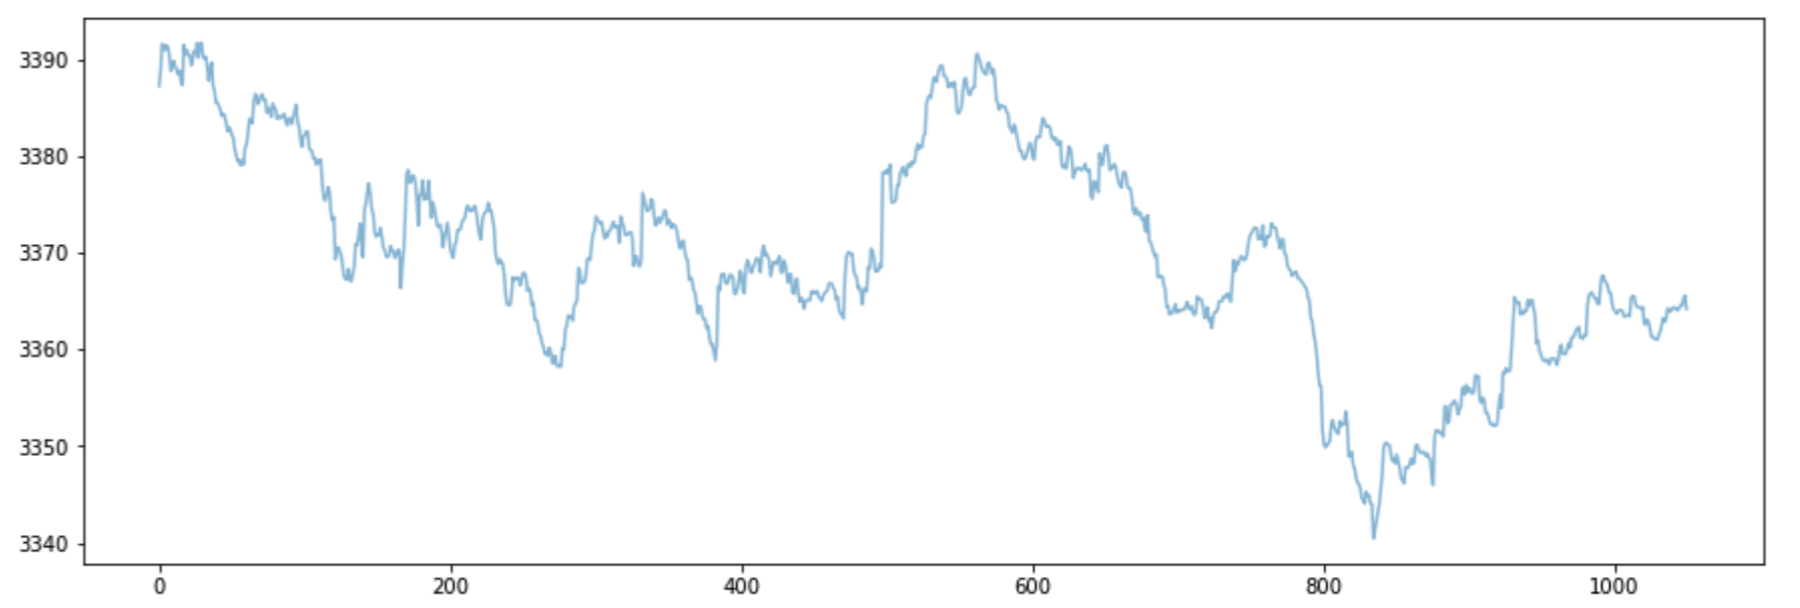
\includegraphics[width=1\textwidth]{../paper/images/stock_example.png}
            \caption{An Example of Stock Price Fluctuations Over Time}
            \label{fig:stock}
        \end{center}
    \end{figure}
    
    
    
\end{frame}



%%%%%%%%%%%%%%%%%%%%%%%%%%%%%%%%%%%%%%%%%%%%
%%%%%%%%%%%%%%%%%%%%%%%%%%%%%%%%%%%%%%%%%%%%

\begin{frame}[fragile]{Buy and Sell advice based on Breakout Patterns of EMA 38 and 100  }


    \begin{figure}
        \begin{center}
            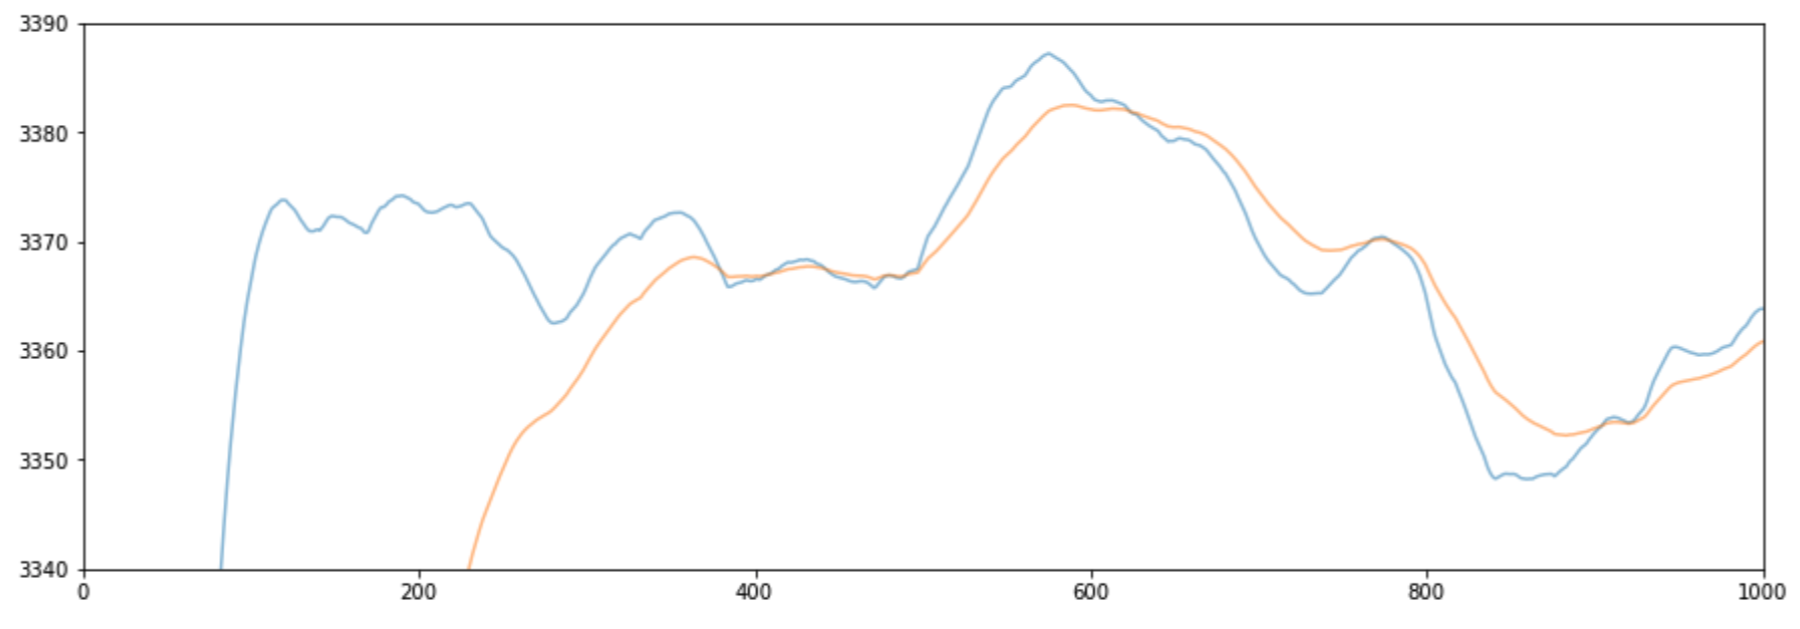
\includegraphics[width=1\textwidth]{../paper/images/query2_example.png}
            \caption{Example of Query 2 - Buy and Sell advice based on Breakout Patterns of EMA 38 and 100}
            \label{fig:EMAs}
         \end{center}
    \end{figure}
    
\end{frame}

%%%%%%%%%%%%%%%%%%%%%%%%%%%%%%%%%%%%%%%%%%%%
%%%%%%%%%%%%%%%%%%%%%%%%%%%%%%%%%%%%%%%%%%%%

\begin{frame}[fragile]{ Use one of the OSS or implement from scratch?}


    Should we use one of the Open Source Stream processing systems like: 
\begin{itemize}
    \item \blueb{Apache Spark - Streaming}
    \item \blueb{Apache Flink - Streaming}
    \item \blueb{Apache Storm}
    \item \blueb{Apache Kafka for streaming pipelines} 
    \item \blueb{Esper Stream processing}
    \item  ... 
\end{itemize}

    We decided to implement the DEBS Grand Challenge from scratch. 
    
    \redb{Why?}
    
        
\end{frame}


%%%%%%%%%%%%%%%%%%%%%%%%%%%%%%%%%%%%%%%%%%%%
%%%%%%%%%%%%%%%%%%%%%%%%%%%%%%%%%%%%%%%%%%%%

\begin{frame}[fragile]{ }





    
\end{frame}


%%%%%%%%%%%%%%%%%%%%%%%%%%%%%%%%%%%%%%%%%%%%
%%%%%%%%%%%%%%%%%%%%%%%%%%%%%%%%%%%%%%%%%%%%

\begin{frame}[fragile]{ }





    
\end{frame}



\end{document}